%! suppress = MissingImport
%%%%%%%%%%%%%%%%%%%%%%%%%%%%%%%%%%%%%%%%%
% Developer CV
% LaTeX Template
% Version 1.0 (28/1/19)
%
% This template originates from:
% http://www.LaTeXTemplates.com
%
% Authors:
% Jan Vorisek (jan@vorisek.me)
% Based on a template by Jan Küster (info@jankuester.com)
% Modified for LaTeX Templates by Vel (vel@LaTeXTemplates.com)
%
% License:
% The MIT License (see included LICENSE file)
%
%%%%%%%%%%%%%%%%%%%%%%%%%%%%%%%%%%%%%%%%%

%----------------------------------------------------------------------------------------
%	PACKAGES AND OTHER DOCUMENT CONFIGURATIONS
%----------------------------------------------------------------------------------------

\documentclass[8pt]{developercv} % Default font size, values from 8-12pt are recommended
\usepackage{enumitem}
\usepackage{tikz}

%----------------------------------------------------------------------------------------
\ifdefined\generated
\else
\newcommand{\generated}{manually}
\fi

\newcommand{\linebreaksmall}{\vspace{2mm}}
\begin{document}

%----------------------------------------------------------------------------------------
%	TITLE AND CONTACT INFORMATION
%----------------------------------------------------------------------------------------

\begin{minipage}[t]{0.5\textwidth} % 50% of the page width for name
	\vspace{-\baselineskip} % Required for vertically aligning minipages
	% If your name is very short, use just one of the lines below
	% If your name is very long, reduce the font size or make the minipage wider and reduce the others proportionately
	\colorbox{black}{{\HUGE\textcolor{white}{\textbf{\MakeUppercase{Maximilian}}}}} % First name
	
	\colorbox{black}{{\HUGE\textcolor{white}{\textbf{\MakeUppercase{Link}}}}} % Last name
	
	\vspace{6pt}
	
	{\large Founding Full-Stack Engineer} % Career or current job title
\end{minipage}
\begin{minipage}[t]{0.3\textwidth} % 30% of the page width for the first row of icons
	\vspace{-\baselineskip} % Required for vertically aligning minipages
	
	% The first parameter is the FontAwesome icon name, the second is the box size and the third is the text
	% Other icons can be found by referring to fontawesome.pdf (supplied with the template) and using the word after \fa in the command for the icon you want
	\icon{MapMarker}{9}{Karlsruhe, Germany}\\
	\icon{Phone}{9}{+49 172 2389581}\\
	\icon{At}{9}{\color{blue}{\href{mailto:contact@mxlink.de}{contact@mxlink.de}}}\\
	\icon{Github}{9}{\color{blue}{\href{https://github.com/mxlnk}{github.com/mxlnk}}}\\
\end{minipage}
\begin{minipage}[t]{0.2\textwidth} % 20% of the page width for the second row of icons
	\vspace{-\baselineskip} % Required for vertically aligning minipages
	\begin{tikzpicture}
		% Draw red border circle
		\draw[darkgray, line width=2pt] (0,0) circle (1.5cm);
		% Clip image to circle
		\begin{scope}
			\clip (0,0) circle (1.5cm);
			\node[anchor=center] at (0,-0.2) {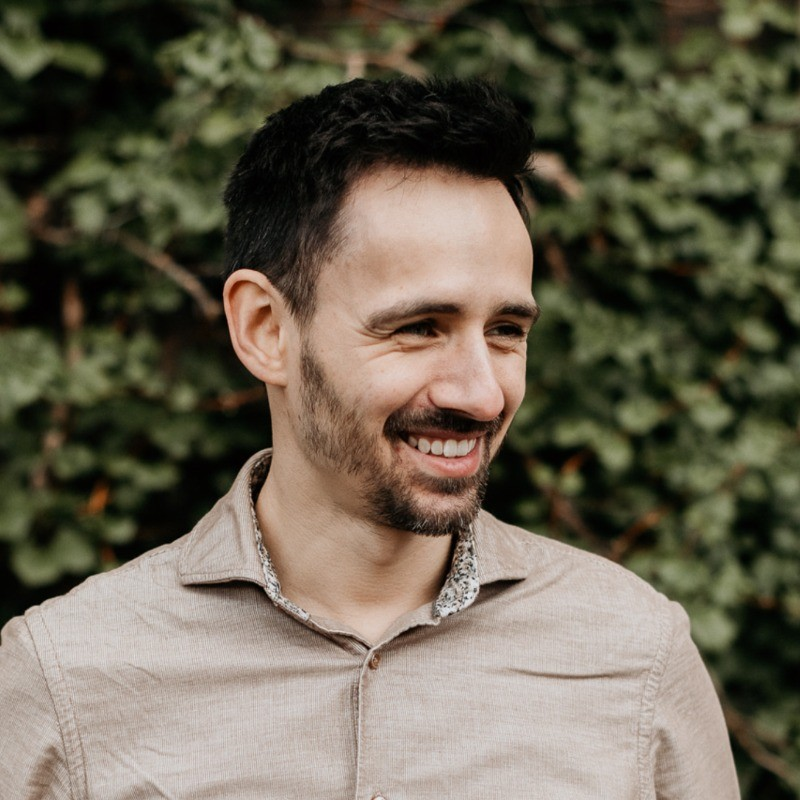
\includegraphics[width=3.5cm]{./profile.jpeg}};
		\end{scope}
		%adjust this coordinate to move image
	\end{tikzpicture}

\end{minipage}

\vspace{0.5cm}

%----------------------------------------------------------------------------------------
%	INTRODUCTION, SKILLS AND TECHNOLOGIES
%----------------------------------------------------------------------------------------


\begin{minipage}[t]{0.45\textwidth} % 45% of the page width for the introduction text
	\vspace{-\baselineskip} % Required for vertically aligning minipages
	\cvsect{Values}

	Agile and pragmatic approach to problem solving. My colleagues value my ability to prevent scope creep and keep the focus on the important things.

	Focused on building the right solution that actually moves the company forward and helps customers.

	Recognized for a positive, constructive approach and openness to feedback.

	Used and proven to being a self-starter and taking ownership.

\end{minipage}
\hfill % Whitespace between
\begin{minipage}[t]{0.45\textwidth} % 45% of the page for the skills bar chart
	\vspace{-\baselineskip} % Required for vertically aligning minipages
	\cvsect{Technology}

	A key technical contributor in two growing startups, working end-to-end across backend services, frontend applications, CI/CD and cloud infrastructure.

	Currently using TypeScript, Node.js, React, PostgreSQL, Google Cloud Platform, Kubernetes and Docker but not limited to these. Always eager to learn new technologies and improve my skills.

	Prior experience with Vue.js, MongoDB and Python.
	
	I highly value maintainable and readable code and strive to eliminate over-engineering and premature optimization.
\end{minipage}

%\begin{center}
%	\bubbles{5/Eclipse, 6/git, 4/Office, 3/Inkscape, 3/Blender}
%\end{center}

%----------------------------------------------------------------------------------------
%	EXPERIENCE
%----------------------------------------------------------------------------------------

\cvsect{Experience}

\begin{entrylist}
	\entry
		{2023 -- Current}
		{Senior Full-Stack Engineer}
		{octomind GmbH}
		{Built SaaS tooling leveraging LLMs, agents, and Playwright to automatically generate, execute, and maintain E2E tests. Main work on React, and Material UI frontend and a backend written in TypeScript and Node.js.
		\begin{itemize}[nosep, topsep=0pt, left=5pt, after=\vspace{6pt}]
			\item Split off long running jobs from our core service to be able to handle increased load of a closeby launch
			\item Live parsing of playwright traces, enabling customers to live view their tests generating
			\item Major refactoring of our monolithic codebase into packages, improving maintainability
			\item Several major bugfixes, e.g. a memory leak severely impacting the stability of our service
			\item Worked closely with customers and product teams to align technical solutions with business goals
		\end{itemize}
		\texttt{TypeScript}\slashsep\texttt{Node.js}\slashsep\texttt{React}\slashsep\texttt{LLMs and Agents}\slashsep\texttt{PostgreSQL}\slashsep\texttt{Docker and Kubernetes}} \linebreaksmall
	\entry
		{2017 -- 2023}
		{Founding Full-Stack Engineer}
		{understandAI GmbH}
		{Joined as first engineer. Built SaaS tooling for the annotation of automotive sensor data, including orchestration of human, AI and algorithmic workloads. Main work on Vue.js based frontends, several backend microservices written in TypeScript and the cloud infrastructure.
		\begin{itemize}[nosep, topsep=0pt, left=5pt, after=\vspace{6pt}]
			\item Led the development of the in-house annotation tool allowing the first customer projects and revenue
			\item Developed major parts of an orchestration service, handling flexible workflows of human, AI and algorithmic workloads allowing for cusomer projects on a huge scale with hundereds of annotators and millions of annotations
			\item Took on challenging and troubled customer project, helping turning the project around and securing the biggest customer to that date
			\item Mentored engineers, supported onboarding, and participated in hiring decisions
			\item Took on team leadership responsibilities and owned major product areas at multiple stages
		\end{itemize}
		 \texttt{TypeScript}\slashsep\texttt{Vue.js}\slashsep\texttt{Node.js}\slashsep\texttt{MongoDB}\slashsep\texttt{Python}\slashsep\texttt{Docker and Kubernetes}} \linebreaksmall
	\entry
		{2014 -- 2017\\\footnotesize{part-time}}
		{Working student software engineering}
		{SearchHaus GmbH}
		{Worked on a knowledge graph search engine in a 4-person startup environment, contributed Java backend service, created Angular.js frontend for knowledge graph exploration and querying.
		\linebreaksmall \\ \texttt{Java}\slashsep\texttt{Spring Boot}\slashsep\texttt{Angular.js}}
\end{entrylist}

%----------------------------------------------------------------------------------------
%	EDUCATION
%----------------------------------------------------------------------------------------

\cvsect{Education}

\begin{entrylist}
	\entry
		{2016 -- 2020}
		{Computer Science, Msc}
		{Karlsruhe Institute of Technology}
		{Focus on machine learning/artificial intelligence classes, especially in the computer vision realm.
		
		Final grade: 1,2. Final thesis \color{blue}{\href{https://ieeexplore.ieee.org/abstract/document/9627069}{paper}}.}
	\entry
		{2012 -- 2016}
		{Computer Science, Bsc}
		{Karlsruhe Institute of Technology}
		{Final grade: 1,9.}
	\entry
		{2012}
		{Abitur}
		{Burghardt-Gymnasium Buchen}
		{Final grade: 1,2.}
\end{entrylist}

%----------------------------------------------------------------------------------------
%	ADDITIONAL INFORMATION
%----------------------------------------------------------------------------------------

\begin{minipage}[t]{0.3\textwidth}
	\vspace{-\baselineskip} % Required for vertically aligning minipages

	\cvsect{Languages}
	\newline
	\textbf{German} - native\\
	\textbf{English} - fluent\\


\end{minipage}
\hfill
\begin{minipage}[t]{0.3\textwidth}
	\vspace{-\baselineskip} % Required for vertically aligning minipages
	
	\cvsect{Personal and Hobbies}
	
	I recently (2024) became a father and love spending time with my family. Otherwise I enjoy hiking and rock climbing.
\end{minipage}
\hfill
\mbox{}
\vfill
\begin{minipage}[t]{1.0\textwidth}
\centering{\footnotesize{This document was generated \generated~on \today. Source Code available on \color{blue}{\href{https://github.com/mxlnk/cv}{github}}.}}

\end{minipage}

%----------------------------------------------------------------------------------------

\end{document}
